\documentclass[11pt]{article}



\usepackage{natbib}
\usepackage{hyperref}
\usepackage{eurosym}
\usepackage{graphicx}

\begin{document}

\setlength{\parindent}{0pt}
%first draw, fmolo, 28.10.2012

\tableofcontents
\section{The debate among economists}

\subsection{China's exports}

Exports of Chinese goods and services to the world market have risen dramatically over the last decade. %include
   
     \begin{figure}[h]
     \begin{center}
     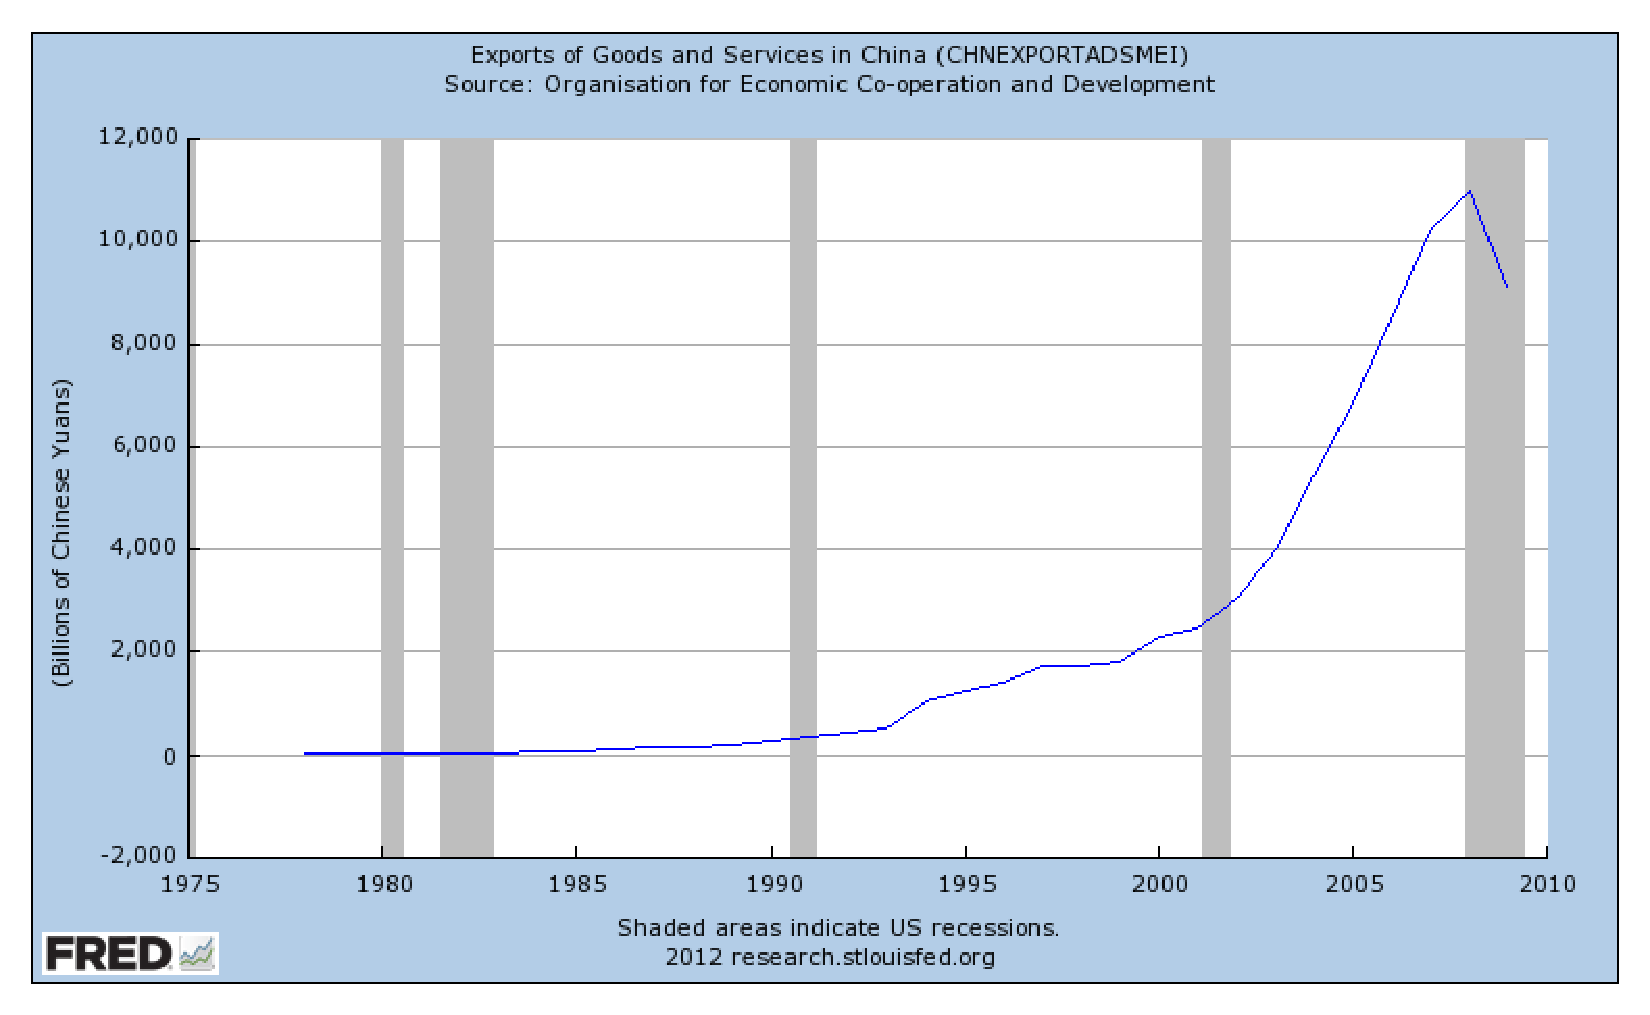
\includegraphics[width=1\textwidth]{ExportsChinaFRED.pdf}
     \end{center}
     \end{figure}

During the same period, imports of foreign goods to China have risen much less. Around the year 2010, China exported much more goods than it imported. In economic terms, China was running a \emph{current account surplus}. In absolute terms, such a current account surplus  is unprecedented. %account surplus data is easily available. including switzerland might be fun, because the Swiss surplus is even higher. China is taking a larger share of the total world production now than it did ten years ago. Therefore, the growth of exports reflects not only the continuing integration of China's economy in the world market but also the high competitiveness of Chinese goods. 

But why are Chinese goods so competitive on the world market? One might be tempted to point out the hard work, innovation and creativity of the Chinese working force.\footnote{As \cite[p. 18]{Yu2010} indirctly does.} Not being convinced by this, economists have brought forward several other, more structural explanations:

One factor is \emph{labor arbitrage}:\footnote{This factor was hinted at by Xu Mingqi of the Institute of World economy of the Shanghai Academy of Social Sciences in a talk to our class on September 4 2012.} Chinese workers are willing to work at lower wages than workers in importing countries. Importantly, accepted wages are not only lower in absolute terms but also in terms of purchasing power: A typical wage in China allows for a lower standard of living than a typical wage in an industrial country, thereby allowing Chinese firms to produce with much lower (absolute and relative) labor costs. 

In addition to cheap labor Chinese producers find other \emph{cheap factors of production}, namely energy and land rents.\footnote{\cite[pp. 25]{Huang2010}.} These markets are not liberalized and prices can therefore be strongly influenced by government policy. Since for Chinese officials - as well on the local as on the federal level - GDP growth is a major ambition, energy and land use prices are cheaper on average than in industrial countries and even cheaper than in other emerging economies.

Another factor explaining strong Chinese exports has been introduced in 2005 by Ben Bernanke, shortly before he was named chairman of the US Federal Reserve.\footnote{\cite{Bernanke2005}}: The \emph{saving glut hypothesis}. According to Bernanke a special series of circumstances has lead to exceptionally high saving rate, i.e. the percentage of income that is saved. These circumstances include repercussions of the financial crises in emerging economies in the late 90's, but also the unique saving behaviour of Chinese households. Partly due to the lack of social security institutions and to the One-Child-Policy, the saving rate of Chinese households is among the highest in the world - in 2007 it was 53\% as opposed to Switzerland's 17,5\%.\footnote{\cite[pp. 20]{Taoyang2011}.}\footnote{Swiss Federal Statistics Office, http://www.bfs.admin.ch/bfs/portal/en/index/themen/00/09/blank/ind42.indicator.420004.420001.html.} These savings drive down interest rates in China and allow the local producers to access very cheap loans, which in turn allows them to expand production.\footnote{This explanation is also favoured by \cite[pp. 41]{Wyplosz2010}.}

Besides all these factors, \emph{China's exchange rate policy} is another factor that might possibly explain part of the competitiveness of Chinese goods. In order to illustrate the relevance of the exchange rate of the Chinese Currency, the renminbi (RMB), we introduce a fictional story about two companies in the next section. The story takes place in a hypothesized world where we assume the RMB to be \emph{undervalued}. 





%\subsection{world market} basic idea: prices of goods. exports and imports. trade balances. current account. financial account. they depend on the following factors: x, y, z. one of these factors is the exchange rate. or: surplus would tend towards zero through the mechanism of currency appreciation (?)

% The other story:
% Let's take a look at the financial account and the current account.  
% The financial acocunt is the investments (capital) flowing in and out 
% of a country while the current account constitutes the trade balance, 
% earnings on foreign investments and cash flows (e.g. remittences).

% Per definition these two accounts balance each other in the sense that 
% if a nation has a trade deficit causing their current account to be 
% negative, the government would have to borrow money or in other words 
% let foreign governments invest in their bonds, creating a financial 
% account surplus.

% China in particular has both a trade surplus and a lot of foreign 
% investment. This leads to an advantagous situation where the National 
% Bank of China ends up with a lot of foreign currency from people 
% buying RMB to buy chinese products or construct factories in China.

% Many of the dollars that are bought by the National Bank of China are 
% reinvested into US state bonds, in effect enabling the US to keep 
% their budget deficit running.

% When the Chinese National Bank sells RMB to investors and trading 
% partners, they are in a sense free to decide how many dollars you 
% would need to buy 10 RMB. However, deciding on the exchange rate has 
% far reaching consequences that we'll get back to.

% Now, what decides the price of a product sold by a company in one 
% country to a company in another?

% 

% The third story:

% How about the following outline:
% Introduce the economy of a country like in Krugman's book as a company 
% investing money and having expenses. Explain the concepts of current 
% account and financial account in terms of these down to earth company 
% expenditures and incomes and differentiate the concepts by outlining 
% how the financial account are items that generate income while the 
% current account are items that don't.

% With this in place transplant the analogy to a country and demonstrate 
% how the different aspects map on to the economics of a country.  
% Introduce why the current account + financial account = 0 and explain 
% intuitively why that is true.

% Of course things don't work in a country like they work for a company, 
% so let's flesh out how different elements of the expenditures and 
% incomes work in a country. In particular explain how:
% - How trade between to companies in different countries work
%	[ If Migros wanted to buy Danish potatoes they would need to get 
%	hold of Danish kroners to pay the Danish farmers first. To get 
%	Danish kroners, they would buy them on the currency exchange where 
%	they would originate from Danish Banks. ...(stop here?) The Danish 
%	Banks in turn get their supply of Danish Kroners from the National 
%	Bank of Denmark. In Denmark the National Bank have decided to peg 
%	the value of the Danish Kroner to the Euro meaning that you can 
%	count on buying around 7.45dkk for 1eur. They 

% - The different shapes of foreign investment
%	[ Foreign investment comes in many shapes and forms. The most 
%	intuitive case is an example where a Swedish company invests money 
%	in a Vietnamese jungle clearing endavour in the hope of future 
%	returns. A big chunk of international investment however is done by 
%	trading state bonds. When i.e. Spain run with a budget deficit they 
%	sponsor this deficit by issuing state bonds, which basically works 
%	as I-owe-you notes with a low interest. Because states rarely fail 
%	as opposed to companies, these bonds are a very secure place in 
%	which to put your foreign currency.

%	Similarly the 


% How does the swiss national bank peg their currency at a certain rate?
 

% In order for foreign markets to buy chinese goods or invest by for 
%example constructing factories in china, they need RMB to pay with. 

% When for example the United states are drafting a new budget they 

\subsection{An illustrative story}

% TODO: Find a way to ident or otherwise mark this section to clearly 
% indicate where the story starts and ends

Based on a very successful prototype, Fluttr, a US mass manufacturer of pop art,  has decided to massproduce 
250000 miniature christmas trees made in parts with porcelain fixtures 
and in their search for a supplier they've come across MingFix, a Chinese porcelain producer,  who can 
produce fixtures at a rate much cheaper than american companies 
producing similar products. A contract is signed and Fluttr owes 
MingFix the net sum of 23 million RMB. However, Fluttr being an american 
company will have to exchange their dollars to RMB to fulfil their part 
of the contract, something they do by selling their dollars to a chinese 
bank.

% For most other currencies it's possible to easily exchange large 
% amounts of money on a currency exchange where the price of the 
% currency fluctuates with the demand and supply. However China retains 
% strict control over the access to RMB and leverages full control over 
% the value of RMB per Dollar. Currently the RMB is pegged at a fixed 
% rate to the US dollar.  This means that the exchange rate between the 
% two economies remains constant over time at 6.24RMB per Dollar. This 
% makes it easy for MingFix to sign the contract with Fluttr since none 
% of them need to worry about fluctuations in the exchange rate.  

Since the RMB is undervaluated in our hypothetic scenario both Fluttr 
and MingFix benefits from trading in RMB. For Fluttr it's advantegous 
because a good exchange rate makes the porcelain fixtures cheaper for 
them to buy, and MingFix benefits because it increases their ability to 
compete on an international market as long as they aren't reliant on 
importing products from the US.

% The dollars from the transaction ends up in the hands of the People's 
% Bank of China who aren't interested in keeping the money as is, since 
% it doesn't give them any interests and constantly loses value due to 
% american inflation. Some of the dollars are sold to Chinese buyers. 
% Some are invested in Chinese projects around the world, but a big 
% chunk of them are put in US federal bonds. These bonds are issued by 
% the US Federal Bank to cover for the trade deficit. From an american 
% viewpoint the bonds are a way to borrow money while they to the 
% Chinese is a secure way to store their american Dollars. Usually the 
% bonds will yield a bit of interest and since they are issued by a 
% nation that is very unlikely to default on its payments it is a very 
% secure way of store the dollars.

The christmas trees were a great succes and Fluttr are looking into out 
sourcing the production and decides to invest in Chinese factory 
facilities in partnership with MingFix. To start production they invest 
42 mllion RMB in China in the form of wages, land rent, buildings 
machinery and laywers typing up contracts.  This money is based on 
Dollars as before, and again the People's bank of China steps in to sell 
RMB to Fluttr for their Dollars.  Both Fluttr and MingFix benefit from a 
cheap exchange rate once again, since this gives them more value for 
their money on Chinese soil.

Half a year down the road Fluttr starts to see their market shares in 
porcelain christmas trees diminishing due to a new Chinese competitor 
calling themselves Flittle and selling similar products much 
cheaper.  While the Dollar RMB exchange rate original benefitted Fluttr, 
they are now at a disadvantage by having large part of their design and 
administration working in the US. This makes their profit margins for 
each product sold much smaller than Flittle who benefits from a cheap 
exchange rate when they export their goods because the dollars their 
consumers pay are exchanged to RMB's at a beneficial rate.

Fluttr are forced to lay off a large part of their staff in the US as a 
response and since none of the executives are willing to relocate to 
China and start a new life there under better circumstances for their 
company, they instead spend their evenings writing angry letters to 
their senators pushing them to put pressure on China to increase the 
value of the RMB. They might have benefitted from the exchange rate for 
a while, they readily admit, but there is no way they can compete with 
an entirely Chinese company and they would much rather give up their 
collaboration with chinese suppliers than competing against chinese 
companies.

% TODO: mark the end of the story


%It's important to remark in this hypothetical case that there can be 
%many more reasons why a Chinese product might be cheaper than an 
%American equivalent, even under the assumption that the RMB is 
%undervalued. However in the counter scenario where the Chinese RMB is 
%not undervaluated, several things change. Fluttr might be less reluctant 
%to enter the Chinese market given that they have less purchasing power 
%per Dollar. It might well be that an alternative American supplier of 
%porcelain fixtures can provide competing prices. This difference is even 
%more pronounced when it comes to investing in Chinese production 
%facilities. Both the initial investment as well as the goods produced by 
%the facilities become more expensive as the RMB increases in value in 
%relation to the American Dollar.

\subsection{Impact of the exchange rate}

The above example illustrates that the exchange rate between the RMB an the US Dollar has 
a very direct impact on american and chinese companies. If the value of the RMB drops by 10\%, the porcelain fixtures of Mingfix and the miniature christmas trees of Flillte for a price 10\% lower than before on the world market and become much more competitive.\footnote{The issue becomes somewhat more complicated when Chinese producers buy components of their products outside of China. The lower value of the RMB makes imports more expensive and offsets part of the price gain. This analysis therefore applies only to products where more than half of the value is added in China, certainly a large part of Chinese exports.} A low-valued RMB might therefore also explain part of the competitiveness of Chinese export goods. 

There is yet another function of the currency exchange rate. Let's look at what happens when Fluttr buys goods from MingFix: they buy RMB from a Chinese commercial bank, paying with US Dollars. They do the same again when they invest in China. But they are not the only ones doing so - if Chinese products, for whichever of the above-mentioned possible reasons, are very competitive, \emph{many} US firms will buy RMB, paying with US Dollars. This drives the demand for RMB on the world market of currencies up. Other things equal, according to very basic supply-demand models of economics, this should drive the price of the RMB up. At the same time, the US Dollars being sold on the market raise the supply of US Dollars and should thereby lower their price. If the currency market was a completely competitive and open market, the exchange rate would always be balanced at a point where demand and supply for RMB are stable - the same for US Dollars. Macroeconomic theory postulates, that for every two currencies at every 
moment, there is such a balanced exchange rate, called the \emph{equilibrium exchange rate}.\footnote{\cite[p. ?]{Krugman}}. If a currency is below this hypothetical rate, it is undervalued. If it is above it, it is overvalued.

If the market for currencies was completely competitive with firms, banks and private persons being able to buy and produce money at will, all exchange rates would always be at their equilibrium rate. But of course money cannot be produced by anyone. It is National Banks that issue money. They and only they can - figuratively speaking - print a discretionary amount of money in their own 
currency.\footnote{The process is somewhat more complicated than 
printing bank notes, but the effect is the same for the purposes of this 
section.}. Doing this they follow a monetary policy. 


%TODO: I think this belongs in the introduction (of the whole report)
%Both the size and fairness 
%of this impact are however heavily disputed on a diplomatic level 
%between China and the US as well as in academic circles.
%To understand these arguments, it's necessary to introduce a few 
%fundamental concepts. We base these concepts on introductory texts in 
%economics that are generally agreed upon in the field of economics.  
%However as will become obvious once we explore the arguments on either 
%side of the debate, even fairly fundamental issues can sometimes be 
%interpreted in more than one way. We will try as best we are able to 
%illustrate these ambiguities in an impartial fashion.


\subsection{Exchange rate policy}

%Money is a tradable good and different currencies can be traded against 
%each other in the foreign exchange market. Market participants such as 
%private persons, corporations, commercial banks and national banks can 
%exchange a certain amount of a currency for another amount of another 
%currency. This exchange takes place either at commercial banks and 
%currency exchanges on an open market with flexible prices (i.e. exchange rates), or by trading 
%with state owned banks under tighter restrictions as e.g. with the RMB. The 
%exchange rate as introduced in the story of Fluttr and MingFix is the
%price of a currency A in terms of currency B. On an open market, the 
%exchange rate is determined by supply and demand for a currency. If at 
%some point the demand for US Dollars rises, for example because a 
%international corporation invests in the US and pays workers there a 
%wage in US dollars, the price of the dollar on the currency market will 
%be higher, i.e. you will get fewer US dollars for one euro. 

The standard monetary policy of western countries is to define a target for inflation, normally around 2\%. The National Banks are mandated to control the supply of money such that this target is met. Currencies of these countries are then traded freely against each other and their exchange rate fluctuates with varying demand. 

But nations can also chose to exercise a tighter control of the value of their 
exchange rate. 
This is very common: Some national banks even use their money 
supply to `peg' their currency to another, so that exchange rates are 
fixed.  For example, the Swiss National Bank (SNB) offers every vendor 
of an euro CHF 1.20 in exchange.  Since the SNB controls the money 
supply of Switzerland, it will never run out of CHF and the exchange 
rate of the Swiss franc. As a consequence the euro will never be lower 
than 1.20 until the SNB changes its exchange rate policy.  As another 
example, the national bank of Denmark controls the supply of Danish 
kronor so that the exchange rate of the kronor and the euro constantly 
remains at 0.134 (with a small bandwith of +/-2.25\%).

In these cases monetary policy becomes exchange rate policy: It does not focus mainly on inflation or other measures but on the exchange rate.

Since manipulating the 
exchange rate can be beneficial for a nation's exports and 
foreign investments, National Banks might feel tempted to promote their country's exports by holding the exchange rate low. However this behaviour forces trading competitors 
to take similar steps in order to protect their own exports, which 
easily leads to a situation where countries are competing to devaluating 
their currencies in order to compete, a policy known as `beggar thy neigbour'. After such an episode during the Great Depression, such behaviour was internationally recognized as nonbeneficial for all partners involved and international 
institutions were instantiated to create a set of rules for all countries and observe if National Banks abide by these rules. The most prominent of these today are the IMF (International 
Monetary Fond), the WTO (World Trade Organization) and the EU (European 
Union).
%TODO: Is this story really true? (there is something in the Krugman textbook somewhere)



\subsection{The case against China's exchange rate policy}

China has been 
accused by prominent US politicians of `manipulating' its currency and 
keeping the Chinese currency, the Renminbi\footnote{abbreviated to CNY. 
The basic unit of the Renminbi is the Yuan.} `undervalued'. This accusation against China can be restated in terms introduced in the previous sections: It claims that China is using monetary policy to keep a 
fixed exchange rate \emph{below} the equilibrium rate. 

\subsubsection{Deviation from the equilibrium exchange rate}

There exists various different theoretical methods for estimating an 
equilibrium exchange rate in the litterature. However, to understand 
them it's necessary to introduce the notion net foreign asset (NFA) as 
well as the concepts of current and foreign account (CA and 
FA)\footnote{For a more in depth explanation \cite{ch.  
18}{KrugmanTextbook} provides a good introduction}.

The net foreign asset is the value of the assets that a country owns 
minus the value of assets from that country which is owned abroad.  
Assets in this sense is usually state bonds but can also be stocks and 
goods.  

The current and financial account are measures for how the NFA changes.  
The current account constitutes the balance of trade and money transfers 
while the financial account constitutes the balance of financial assets, 
that is the debt or amount of money lent to other countries. 
%fmolo: could this be related to the "export success story" i've told in the first section?

The two accounts are related by the current account plus the financial 
accout being equal to zero. This makes sense intuitively since if a 
nation buys more goods than it can finance with exports it needs to 
finance this by selling state bonds instead. In this case, the negative 
trade balance translates to a current account deficit, while the influx 
of money coming from the sale of state bonds translates to a finance 
account surplus.

When it comes to estimating the equilibrium exchange rate these three 
measures are heavily used because they gives us an idea of how stable an 
economy is, judging from how assets and goods are flowing in and out of 
the economy. In particular a report was released in 2008 by the 
Internation Monetary Fund outlining three methods that can be used to 
estimate the disparity between the real and equilibrated exchange 
rate\footnote{The Report: \cite{pp.  1}{Lee08}}:

\begin{enumerate}
\item{The macroeconomic balance approach looks at projections of a 
	country's current account and tries to estimate how much the 
exchange rate would need to be adjusted for it to stabilize within a 
certain level}
\item{The reduced-form equilibrium real exchange rate approach tries to 
	estimate the equilibrium directly as a function of the NFA as well 
as a number of trade indicators}
\item{The external sustainability approach tries to find the exchange 
	rate that would stabilize the NFA of a country to within a certain 
level}
\end{enumerate}

In practice these techniques has been used by Cline and Williamson in 
their yearly policy brief on equilibrium exchange 
rates\footnote{\cite{cline2009,cline2012}}.  Their estimates are based 
largely on the first and third methods proposed by the IMF, designating 
debt and trade surplus above 3\% of GDP as abnormal and calculating how 
much the exchange rate would have to change to bring the current account 
within a normal treshold. In 2009 their results showed that the Chinese 
RMB was undervaluated by 21.4\%, a number which has been much quoted 
since then. Especially in relation to the fact that they found the US 
dollar 17.4\% percent overvaluated, futher contrasting the value gap 
between the two currencies.

%fmolo: i don't understand the method that follows
% 
Instead of trying to find the equilibrium exchange rate, a different 
approach is to do the exact opposite. If we pick a comparative point in 
time or statistical measures based on other countries, we can measure 
how much the current exchange rate deviates from a factor that remains 
constant.

If we pick the unit price of labour as our constant and 1998 as our 
point of reference it is straightforward to show that the RMB is 25 
percent undervalued when compared to at least the American 
Dollar\footnote{\cite{chimerica2009}}. Similarly we can focus on the 
purchasing power parity (PPP)\footnote{The PPP is a measure for how the 
price for similar goods and services in two countries differ}. Based on 
the behaviour of poor countries in growth based on the PPP, it is 
estimated that the RMB is undervalued between 12\% and 
47\%\footnote{\cite{Subramanian2010}}.

% It's really funny that this text (Subramanian2010) is quoting Cline 
% and Williamson as well as Goldstein and Lardy for agreeing on the same 
% number, when in fact Goldstein and Lardy have their number from Cline 
% and Williamson (2009)

% Also from the same paper:
% Since each of the four estimates suffers from limitations, a 
% reasonable approach would be to average all four. This yields an 
% undervaluation estimate for China of about 31\% against the dollar, 
% which is my preferred PPP-based estimate.
% who are giving grants to these people?
%fmolo: awasn't me

\subsubsection{Circumstantial evidence for RMB manipulation}

Estimating the equilibrium exchange rate is hard and different methods lead to different results. Critics of China's monetary policy therefore often supplement their model-based estimates with a more theory-based circumstantial case. The structure of this argument is to ask what a National Bank would do according to textbook economics if it were trying to manipulate its currency and then to point out that China is doing exactly (or roughly) this. 


So how would a National Bank keep a rate below its equilibrium rate? According to 
textbook economics this can be done in three ways:\footnote{\cite[pp. 
514]{Krugman2008}}

\begin{enumerate}
\item{The government can shift supply and demand for its currency by intervening on the foreign exchange market. Buying foreign exchange and selling the local currency drives the price of foreign exchange up and that of the local currency down.}
\item{The government can shift supply and demand by means of monetary policy, namely by keeping interest rates low. Lower interest rates mean lower returns for foreign investors. If foreign investors refrain from investing locally, the demand for the local currency decreases, driving the price of the local currency down.}
\item{The government can impose foreign exchange controls, forbidding foreigners to buy the local currency, therefore again reducing demand and therefore the price of that currency.}
\end{enumerate}

According to Goldstein and Lardy\footnote{\cite[pp.  
40]{GoldsteinLardy2008}}  this is what the People's Bank of China has been doing for a decade:

\begin{enumerate}
\item{The Chinese government has intervened on the foreign currency 
		market on a massive scale: It has been buying foreign 
		currencies, mainly US Dollars (in the form of US government 
		debt) in exchange for RMB to the amount of 10\% of its GDP, i.e. 
		10\% of the value of all goods and services produced in China.} 
		%show data. but first find data (IMF? FRED?)
\item{Interest rates in China are relatively low: When the interest rate is adjusted for inflation, the so called \emph{real} interest rate, interest rates have actually being negative for the most part since 2006.} %show data. but first find data (World Bank?)
\item{China imposes foreign exchange controls that prevent international investors or other governments to buy RMB.}%this seems clear, but i have not yet found how they do it exactly
\end{enumerate}

As a result, critics of Chinas exchange rate regime say, China's export sector has become extremely competitive. 


But the circumstantial evidence goes further than this. If the Chinese government buys foreign currency paying with RMB, it is increasing the amount of money in the economy.\footnote{In economical jargon it is expanding the \emph{monetary base}, what (other things equal) leads to an increase in money supply} Again according to standard economic models\footnote{\cite[pp. ?]{Krugman2008}} an increase in the money supply raises the price level in the domestic economy, leading to inflation.\footnote{Maybe quickly explain the assumed mechanism?} As a result, goods produced in China would become more expensive on the world market not due to currency appreciation, but because production costs (e.g. wages of Chinese workers) rise with inflation. According to this model, even though the People's Bank of China (PBC) keeps the \emph{nominal} exchange rate fixed, the \emph{real} exchange rate, i.e. the exchange rate would float.\footnote{\cite[p. 509]{Krugman}} Therefore, inflation would in the long run offset the competitive advantage of Chinese goods on the world market gained by the low(er) nominal value of the RMB.

%e.g. wang2011 (BIS) mentions sterilisation

China has indeed seen some inflation during the last ten years. But it was only moderatly higher than in other countries - the real and the nominal exchange rate roughly moved in unison during the last ten years.\footnote{source: http://www.clevelandfed.org/research/trends/2010/1110/01intmar.cfm}%TODO: find data to display
Critics of China attribute this to China's \emph{sterilization} of the money inflows. Since 2003, China hast prevented about 40\% of the money inflows of entering the monetary base by raising reserve requirements of Chinese commercial banks.\footnote{IMF, via Cleveland Fed, http://www.clevelandfed.org/research/trends/2010/1110/01intmar.cfm}%display data?
Raising reserve requirements limits the amount of loans the commercial banks can issue, therefore 'extracting' money out of the economy. This in turn limits inflation and prevents the real value of the RMB to rise. This is another manifestation of China manipulating the RMB exchange rate: Not only does it keep the nominal exchange rate artificially low, it also intervenes on the real exchange rate, preventing the 'natural' offset on nominal currency manipulation.

\subsubsection{In the name of the Chinese people}


%TODO: Find (remember) sources/quotations for this:
Critics of China sometimes supplement their case with the assertion, that a higher-valued RMB would actually be in the interest oft the Chinese people, if not its export sector.

First, for an ordinary Chinese factory worker, having a cheap RMB might on one hand mean that their factory 
is doing great on foreign markets, but at the same time buying foreign 
products like European cars or American gadgets becomes very expensive. 

Second, artificially low interest rates, in combination with inflation, deprive Chinese citizens of attractive saving options on their bank accounts. Due to capital controls they cannot place their money in foreign banks where interest rates are higher. In absence of a comprehensive social welfare state, retirement provisions become a major concern for many citizens.

Third, lacking other saving opportunities, many Chinese invest their money in real estate as a saving asset, driving real estate prices up. This not only has macroeconomic risks of overheating int the construction sector, but primarily confronts less affluent citizens with serious difficulties to find habitation in urban areas. Infamously high housing prices, e.g. in Shanghai, have become a major social issue, also reflected in popular culture. %TODO: Cite movies (one of them seen in the Summer School), otherwise scrap the last part.



\subsection{Replies in favor of China's exchange rate policy}

Many economists are more sceptical if the RMB is indeed undervalued. We present first the arguments attacking the above-mentioned estimates of equilibrium exchange rates, followed by the arguments responding to the more circumstantial evidence for manipulation of the RMB.

\subsubsection{Difficulties in estimating the equilibrium exchange rate}

The equilibrium exchange rate is an elusive concept.\footnote{\cite[p. 16]{Yu2010}.} Different methods of measuring result in different estimates of the RMB's deviation. 


%TODO: Maybe list the different methods again and point out their difficulties?



\subsubsection{Circumstantial evidence against RMB manipulation}

The reply to the more circumstatial case against China's policy is at the same time more difficult and easier to make than the case against estimations of the equilibrium exchange rate. It is difficult because the case is based on textbook macroeconomic reasoning and nobody disputes that the People's Bank of China is actually taking measures suited to lower the price of the RMB: The accumulated Dollar reserves, low interest rates and capital controls cannot be questioned.

But the reply is also easier because the case against China itself is not completely clear and the alleged undervaluation of the RMB is not quantified. It is based on many  `judgement calls' and as such it is vulnerable.\footnote{\cite[p. 85]{CheungChinnFujii2010}}

In addition there are equally circumstantial cases to make against a alleged RMB undervaluation. First, as pointed out in the first section of this chapter, China's export success can be explained with a variety of factors.  Different authors point to different reasons: Huang Yiping focuses on factor cost distortions.\footnote{Huang2010, http://www.voxeu.org/article/china-us-and-renminbi-rejoinder-krugman} Charles Wyplosz's and Helmut Reisen's focus is on the high saving rate in China.\footnote{\cite[pp. 40]{Wyplosz2010} and \cite{p. 65}{Reisen2010}}. What they have in common is the insistence that there is no need to invoke the alleged RMB undervaluation to explain China's success on the export market.

Second, one might point out the symmetry of the world market.\footnote{\cite[pp. 39-40]{Wyplosz2010}.} While China is running a current account surplus, the US in turn run a current account deficit. According to Wyplosz, this deficit is caused by the low saving rate of US households and the budged deficit of the US government. Instead of trying to explain China's export success with the alleged undervaluation of the RMB, one could with equal justification explain the US deficit with the \emph{over}valuation of the US Dollar. 

Third, each of the practices taken by the POBC may also have legitimate purposes. China is no the only country that pegs its currency to another currency - we already mentioned Switzerland and Denmark doing so. A fixed exchange rate has the advantage of giving firms and consumers certainty about the future value of a currency.\footnote{\cite[p. 515]{Krugman2008}} Lowering interest rates to spur growth is also a tool widely used by National Banks worldwide. And limiting inflation is considered to be one of the main goals of \emph{any} National Bank.\footnote{China's capital controls might be the only exception, but their importance pales against that of China's foreign exchange reserves.}. Finally, many other countries - among them Japan, Germany and Switzerland - run current account surpluses that are as big as China's, relative to their GDP.

%fmolo: The difference could be this: is monetary policy used for normal goals (like controlling inflation) or is it used to manipulate the currency? for some countries these goals align (switzerland), but not so for china (inflation is high, and they still sell RMB)

\subsubsection{it is over}

The last point to make against the accusations against China is extremely straight-forward: Even if the RMB was undervalued in the past, it is not so any more. Even some of the most ardent critics of China's exchange rate policy now reach this conclusion.\footnote{\cite{Krugman2012}http://krugman.blogs.nytimes.com/2012/10/22/an-issue-whose-time-has-passed/ and \cite{ClineWilliamson2012}} %krugman has graphs but doesn't indicate the source. TODO: show data

%We could therefore turn to the question if this adjustment is due to diplomatic pressure ot the US.


\subsection{Wrap up: Up to 15\% or more}

%on each side there are data-driven arguments. but lack of generally acknowledged models results in varying estimates. their value is hard to assess, but given the uncertainties I find this case against China not convincing.

%then there are arguments arguing with theoretical models/mechanisms. It assesses each element of Chinese XR-policy in itself. For every element there might be legitimate reasons. Taken together I agree with Frankel: It is hard to imagine a clearer case of XR manipulation, even though it is not VERY clear.

\end{document}

%TODO: Mention the complaints of other East Asian countries somewhere. e.g. Herrero/Koivu in Evenett
